% =============================================================================
% Reporte final de Procesamiento del Lenguaje Natural
% Recuperación de documentos con razonamiento temporal (RETECO, SemEval-2027 Task 1, track 1 TEMPO)
%
% Compilación:  tectonic reporte.tex        (o pdflatex + bibtex + pdflatex x2)
% Versión Word: se genera con pandoc a partir de este archivo (ver README del reporte).
% Las decisiones se tomaron en train; dev se usó una sola vez, al final (sección sec:res-dev).
% =============================================================================
\documentclass[11pt,a4paper]{article}

\usepackage{iftex}
% Con pdfLaTeX se usa inputenc/fontenc; con XeLaTeX o LuaLaTeX (p. ej. tectonic), fontspec.
\ifPDFTeX
  \usepackage[utf8]{inputenc}
  \usepackage[T1]{fontenc}
  \usepackage{lmodern}
\else
  \usepackage{fontspec}
\fi
\usepackage[spanish,es-tabla,es-noquoting]{babel}
\usepackage[margin=2.5cm]{geometry}
\usepackage{amsmath,amssymb}
\usepackage{booktabs}
\usepackage{graphicx}
\usepackage[round,authoryear]{natbib}
\usepackage[hidelinks]{hyperref}
\usepackage{url}

\title{Recuperación de documentos con razonamiento temporal en TEMPO:\\
limpieza de consultas, embeddings y fusión híbrida}
\author{Cruz Mendoza Valentina Ayelen\\
Monroy Villegas Isaac\\
{\small Instituto de Investigaciones en Matemáticas Aplicadas y en Sistemas (IIMAS), UNAM}\\
Procesamiento del Lenguaje Natural --- Proyecto final}
\date{Noviembre de 2026}

\begin{document}
\maketitle

% -----------------------------------------------------------------------------
\begin{abstract}
Trabajamos sobre el track~1 de RETECO, la Tarea~1 de SemEval-2027, basado en el benchmark TEMPO \citep{abdallah2026tempo}: dada una pregunta de StackExchange que exige razonar sobre el tiempo, hay que recuperar los documentos que la responden dentro del corpus de su dominio (13 dominios, 1.17~M documentos). Usamos solo técnicas vistas en la materia ---expresiones regulares, TF-IDF, embeddings, n-gramas, Jaccard y cadenas de Markov--- y BM25 como variante de TF-IDF. Partiendo del baseline oficial (macro nDCG@10 en train de 0.1075 en la subtarea 1a y 0.1024 en la 1b), mostramos que limpiar y acortar la consulta con expresiones regulares ya sube el resultado a 0.1528 y 0.1660 sin ningún modelo; que un recuperador de embeddings (\texttt{bge-base-en-v1.5}) lo lleva a 0.2277 y 0.2449; y que su fusión con BM25 a medio peso mediante \emph{Reciprocal Rank Fusion} alcanza 0.2367 y 0.2610, es decir, 2.2 y 2.5 veces el baseline. En una única comprobación en dev, con la configuración fijada en train, el híbrido obtiene 0.2519 y 0.2971 (2.2 y 2.5 veces el baseline en dev) y supera al recuperador denso solo de forma significativa en ambas subtareas. Además evaluamos cuatro formas de usar el tiempo o el tipo de razonamiento de forma explícita: enrutar la consulta según su clase de razonamiento, buscar un vocabulario de documento por clase, añadir la década y el siglo de las fechas de la consulta y estimar un perfil temporal implícito con n-gramas y una cadena de Markov, adaptado del \emph{document focus time} de \citet{jatowt2013focus}. Ninguna mejora de forma estable al sistema híbrido, y analizamos por qué.
\end{abstract}

% -----------------------------------------------------------------------------
\section{Introducción}

Muchas necesidades de información reales dependen del tiempo: qué se sabía de algo antes de cierta fecha, cuándo cambió una regla o cómo evolucionó un fenómeno. TEMPO \citep{abdallah2026tempo} es un benchmark de recuperación que reúne este tipo de preguntas, tomadas de 13 comunidades de StackExchange, y que exige razonar sobre el tiempo para encontrar la evidencia. En el paper original, el mejor de 12 recuperadores solo llega a 32.0 de nDCG@10, y BM25 se queda en 10.8. El track~1 de RETECO, la Tarea~1 de SemEval-2027 \citep{reteco2027}, usa ese benchmark con dos subtareas: en la \textbf{1a} se busca con la consulta completa, y en la \textbf{1b} con cada uno de los pasos en que viene descompuesta.

El objetivo del proyecto es mejorar la primera etapa de recuperación usando solo las técnicas de la materia. Nuestras contribuciones son:
\begin{enumerate}
  \item Un análisis exploratorio que identifica el problema principal: el desajuste de vocabulario entre la consulta y los documentos relevantes, más que la falta de razonamiento temporal (sección~\ref{sec:eda}).
  \item Una secuencia de mejoras medida con un protocolo estricto (sección~\ref{sec:protocolo}): variantes de consulta construidas con expresiones regulares, un recuperador de embeddings y su fusión híbrida con BM25 (secciones \ref{sec:metodos} y~\ref{sec:resultados}).
  \item Cuatro experimentos que intentan usar el tiempo o el tipo de razonamiento de forma explícita, con sus controles, y un análisis de por qué no aportan sobre el sistema híbrido (secciones \ref{sec:res-razonamiento}--\ref{sec:res-tt0} y~\ref{sec:discusion}).
\end{enumerate}

% -----------------------------------------------------------------------------
\section{Trabajo relacionado}

\paragraph{TEMPO.} \citet{abdallah2026tempo} construyen el benchmark con 1,730 consultas, 3,976 pasos de recuperación y corpus por dominio, y evalúan 12 recuperadores: léxicos (BM25, 10.8 de nDCG@10), densos de menos de 1B de parámetros (21--25), densos grandes (23--30) y recuperadores orientados a razonamiento (hasta 32.0, DiVeR). También estudian variantes de la consulta: quitar las expresiones temporales apenas cambia el resultado; dejar solo la información temporal lo hunde; y añadir etiquetas temporales estructuradas (intención y anclas) solo ayuda a un modelo que sigue instrucciones. En la descomposición por pasos, el paso aislado rinde mucho peor que el paso junto con la consulta. Estas observaciones guiaron nuestras variantes de consulta y los oráculos de la sección~\ref{sec:oraculos}.

\paragraph{Recuperación léxica.} TF-IDF pondera cada término por su frecuencia en el documento y por la rareza del término en la colección \citep{sparckjones1972statistical,salton1988term}. BM25 \citep{robertson1994okapi,robertson2009probabilistic} es una variante de TF-IDF que satura la frecuencia del término y la normaliza por la longitud del documento. El baseline oficial de la tarea usa la fórmula de \texttt{LuceneBM25Model} de gensim \citep{rehurek2010gensim} con el analizador de Lucene de Pyserini \citep{lin2021pyserini}, que incluye el \emph{stemmer} de \citet{porter1980algorithm}.

\paragraph{Embeddings.} Los recuperadores densos representan consulta y documento como vectores y buscan por similitud, con la misma idea que los embeddings de palabras como word2vec \citep{mikolov2013distributed}: textos con significado parecido quedan cerca en el espacio vectorial. Usamos BGE \citep{xiao2024cpack}, una familia de modelos de embeddings de propósito general, a través de la biblioteca \texttt{sentence-transformers} \citep{reimers2019sentence}. Por dentro, BGE es un codificador \emph{transformer} \citep{vaswani2017attention} del tipo de BERT \citep{devlin2019bert}, preentrenado por sus autores. Nosotros lo usamos como caja negra, igual que un modelo de word2vec ya entrenado: solo le pedimos el vector de cada texto, sin ajustarlo ni modificarlo, y no dependemos de los detalles de su arquitectura. HyDE \citep{gao2023precise} propone buscar con una respuesta hipotética en lugar de con la pregunta; nosotros solo medimos su techo con la respuesta real (sección~\ref{sec:oraculos}).

\paragraph{Fusión de rankings.} \emph{Reciprocal Rank Fusion} (RRF) combina rankings usando solo la posición de cada documento, sin necesidad de que los scores sean comparables \citep{cormack2009reciprocal}.

\paragraph{Tiempo implícito en el texto.} \citet{jatowt2013focus} definen el \emph{focus time} de un documento como el periodo del que habla su contenido, distinto de su fecha de creación. Lo estiman aprendiendo de una colección con fechas explícitas cuánto se asocia cada palabra con cada año, mediante el coeficiente de Jaccard entre las oraciones que contienen la palabra y las que contienen el año; después agregan esas asociaciones en el documento. Con solo palabras el error es de unos 20 años; combinadas con las fechas explícitas, baja \citep[ver también][]{jatowt2015generic}. En su discusión proponen comparar la representación temporal de la consulta con la del documento, que es lo que hacemos en el experimento TT0. TG-RAG \citep{han2025tgrag} representa el corpus como un grafo de hechos con su fecha, organizado en una jerarquía de tiempo, para responder preguntas sensibles al tiempo; de ahí tomamos la idea de modelar la relación entre palabras y periodos como un paso por un grafo, que en TT0 se concreta en una cadena de Markov de un paso.

% -----------------------------------------------------------------------------
\section{Datos, tarea y protocolo}
\label{sec:protocolo}

\paragraph{Datos.} Hay 13 dominios: \texttt{bitcoin}, \texttt{cardano}, \texttt{economics}, \texttt{genealogy}, \texttt{history}, \texttt{hsm} (historia de la ciencia y las matemáticas), \texttt{iota}, \texttt{law}, \texttt{monero}, \texttt{politics}, \texttt{quant}, \texttt{travel} y \texttt{workplace}. En total suman 1,167,159 documentos. Train tiene 1,211 consultas (1a) y 2,762 pasos (1b); el número por dominio va de 7 consultas en \texttt{iota} a 561 en \texttt{history} (tabla~\ref{tab:dominios}). Cada consulta trae además la respuesta aceptada de StackExchange y metadatos (\texttt{guidance}: clase de razonamiento temporal, intención, anclas, un resumen y un plan de búsqueda) que los autores de TEMPO generaron con GPT-4o \citep{openai2024gpt4o} a partir de la consulta y revisaron a mano en una muestra de 200 consultas \citep{abdallah2026tempo}. Ninguno de los dos estará en test.

\paragraph{Métrica.} La métrica oficial es nDCG@10 \citep{jarvelin2002cumulated}: para cada consulta,
\begin{equation}
\mathrm{DCG@10} = \sum_{i=1}^{10} \frac{\mathrm{rel}_i}{\log_2(i+1)}, \qquad
\mathrm{nDCG@10} = \frac{\mathrm{DCG@10}}{\mathrm{IDCG@10}},
\end{equation}
donde $\mathrm{rel}_i \in \{0,1\}$ indica si el documento en la posición $i$ es relevante e IDCG es el DCG del ranking ideal. Se promedia dentro de cada dominio y luego entre los 13 dominios (\emph{macro}), así que \texttt{iota}, con 7 consultas, pesa lo mismo que \texttt{history}. Informamos también el recall a 100 y a 1000 (R@100, R@1000), que mide qué parte de los relevantes llega a la lista de candidatos. Todo se evalúa con \texttt{pytrec\_eval} \citep{vangysel2018pytreceval}, la misma biblioteca que el evaluador oficial.

\paragraph{Protocolo.} Todas las decisiones se toman en train; dev queda reservado para una única comprobación final, que se hizo al final del proyecto con la configuración ya fijada (sección~\ref{sec:res-dev}). En la búsqueda nunca se usan el formato de los identificadores de los documentos (que delata a los relevantes, sección~\ref{sec:eda}), la respuesta aceptada ni \texttt{guidance}; estos campos solo se usan para medir techos (oráculos) y para analizar. Una mejora se acepta si cumple tres condiciones frente a la referencia:
\begin{itemize}
  \item $\Delta$ macro nDCG@10 $\geq +0.01$;
  \item $p < 0.05$ en un test pareado de aleatorización \citep{smucker2007comparison}: bajo la hipótesis nula se invierte al azar el signo de la diferencia de cada consulta y se recalcula la diferencia macro (10,000 permutaciones, bilateral);
  \item mejora en al menos 8 de los 13 dominios.
\end{itemize}

% -----------------------------------------------------------------------------
\section{Análisis exploratorio}
\label{sec:eda}

Antes de diseñar los experimentos analizamos el corpus, las consultas y el baseline. Los hallazgos que más influyeron fueron:

\begin{itemize}
  \item \textbf{Consultas largas y con ruido.} La mediana es de 127 palabras sin HTML (p99: 673), y el HTML ocupa entre el 4~\% y el 21~\% de los caracteres. Un usuario típico escribe de 3 a 10 palabras; los términos clave se diluyen.
  \item \textbf{Desajuste de vocabulario.} Medimos el coeficiente de Jaccard \citep{jaccard1912distribution} entre el conjunto de términos de la consulta y el de cada documento relevante: es de $\approx 0.07$, frente a $\approx 0.025$ con documentos al azar. Los relevantes comparten más vocabulario, pero muy poco en términos absolutos. El baseline no encuentra ningún relevante en su top-1000 en el 44.6~\% de las consultas de \texttt{history}, y su R@1000 macro es de 0.640.
  \item \textbf{El tiempo explícito no separa relevantes de no relevantes.} Con expresiones regulares contamos años, fechas, décadas y siglos en los documentos. La densidad temporal distingue relevantes de no relevantes con un AUC de solo 0.57, y en algunos dominios los relevantes tienen \emph{menos} años que el resto. Según las anotaciones de \texttt{guidance}, solo el 45~\% de los pares (consulta, documento relevante) comparte algún año.
  \item \textbf{Pasos formulaicos.} Los pasos de 1b son instrucciones imperativas cortas (13--17 palabras), y 15 verbos (``identify'', ``search'', ``analyze''\ldots) inician el 97~\% de ellos. Palabras como ``primary sources'' u ``official documentation'' no aparecen en los documentos relevantes.
  \item \textbf{Casi-duplicados.} Con MinHash y LSH \citep{broder1997resemblance,indyk1998approximate}, que estiman el Jaccard entre todos los pares sin compararlos uno a uno, encontramos que entre el 9~\% y el 11~\% de los documentos de los dominios pequeños tiene un gemelo con Jaccard $\geq 0.8$.
  \item \textbf{Un artefacto que no usamos.} Todos los documentos relevantes tienen un identificador con formato corto, y los de formato largo (el 67~\% del corpus) llevan el número de una consulta. Un sistema que lo aprovechara descartaría dos tercios del corpus sin perder ningún relevante, pero es un artefacto de la construcción del dataset, así que no lo usamos.
\end{itemize}

La conclusión del análisis es que el cuello de botella está en la primera etapa y que el problema es sobre todo de vocabulario del tema. Por eso empezamos limpiando la consulta y añadiendo un recuperador semántico antes de atacar el tiempo.

% -----------------------------------------------------------------------------
\section{Métodos}
\label{sec:metodos}

\subsection{Baseline: BM25 oficial}
\label{sec:bm25}

Reimplementamos el baseline oficial con matrices dispersas y reproducimos exactamente sus cifras (0.1075 en 1a y 0.1024 en 1b). Cada texto pasa por el analizador de Lucene (minúsculas, sin palabras vacías y con el \emph{stemmer} de Porter). El peso de un término $t$ en un documento $d$ es
\begin{equation}
w(t,d) = \mathrm{idf}(t)\,\frac{\mathit{tf}_{t,d}}{\mathit{tf}_{t,d} + k_1\left(1 - b + b\,\frac{|d|}{\overline{|d|}}\right)}, \qquad
\mathrm{idf}(t) = \ln\!\left(1 + \frac{N - \mathit{df}_t + 0.5}{\mathit{df}_t + 0.5}\right),
\end{equation}
con $k_1 = 0.9$ y $b = 0.4$, donde $N$ es el número de documentos del dominio y $\mathit{df}_t$ el número de documentos que contienen $t$. La consulta recibe el mismo peso y el score es $s(q,d) = \sum_{t \in q \cap d} w(t,q)\, w(t,d)$. Es TF-IDF con la frecuencia saturada por $k_1$ y normalizada por la longitud mediante $b$. El baseline busca con la consulta cruda, con su HTML, en 1a, y con la consulta seguida de \texttt{"Step:"} y la instrucción del paso en 1b.

\subsection{Variantes de consulta con expresiones regulares}
\label{sec:variantes}

Construimos variantes de la consulta sin ningún modelo:
\begin{itemize}
  \item \texttt{limpia}: título y cuerpo sin HTML.
  \item \texttt{titulo}: solo el título de la pregunta.
  \item \texttt{titulo+inicio}: el título y las primeras 64 palabras del cuerpo.
  \item \texttt{rrf(limpia,titulo)}: se busca con los dos textos y se fusionan los dos rankings con RRF (sección~\ref{sec:hibrido}).
  \item Para 1b, \texttt{paso\_limpio}: con dos expresiones regulares se quitan al paso el verbo imperativo inicial (``search for'', ``identify and analyze'', ``cross-reference findings with''\ldots) y las palabras meta del generador (``primary sources on'', ``official documentation of'', ``focusing on temporal\ldots''). Por ejemplo, ``Search for primary sources on the 1848 revolutions'' queda en ``the 1848 revolutions''. La variante \texttt{titulo+paso\_limpio} concatena el título de la consulta con el paso limpio.
\end{itemize}

\subsection{Recuperador de embeddings}
\label{sec:denso}

Usamos \texttt{bge-base-en-v1.5} \citep{xiao2024cpack}, que produce vectores de 768 dimensiones. Es un codificador \emph{transformer} preentrenado que usamos tal cual, sin ajuste fino, solo para obtener los embeddings (ver la sección de trabajo relacionado). Como entre el 9~\% y el 18~\% de los documentos supera los 512 tokens, cada documento se parte en trozos de 254 tokens con un solape de 30, con un máximo de 4 trozos (los primeros $\sim$1,000 tokens). Los vectores se normalizan, y el score de un documento es el de su mejor trozo:
\begin{equation}
s(q,d) = \max_{c \in \mathrm{trozos}(d)} \mathbf{e}(p \oplus q)^{\top}\, \mathbf{e}(c),
\end{equation}
donde $\mathbf{e}(\cdot)$ es el embedding normalizado y $p$ el prefijo de búsqueda que recomienda el modelo (``Represent this sentence for searching relevant passages:''). Codificar el corpus completo produjo 1.87~M trozos y tardó unas 4.6 horas en un M2 Pro. La búsqueda es exacta, por producto escalar.

\subsection{Fusión híbrida}
\label{sec:hibrido}

El híbrido combina el ranking de BM25 y el del recuperador denso, cada uno con su mejor variante de consulta, mediante RRF ponderado:
\begin{equation}
s(d) = \sum_{i} \frac{w_i}{k + \mathrm{rank}_i(d)}, \qquad k = 60,
\end{equation}
donde $\mathrm{rank}_i(d)$ es la posición del documento en el ranking $i$ (los que no aparecen no suman). El denso pesa $w = 1$ y barremos el peso de BM25 entre 0.2 y 1.

\subsection{Oráculos y clasificación del tipo de razonamiento}
\label{sec:oraculos}

Los oráculos usan información que no estará en test. No son sistemas: sirven para medir el techo de una idea antes de construirla.
\begin{itemize}
  \item \textbf{O1}: buscar con la respuesta aceptada real, el techo de HyDE \citep{gao2023precise}.
  \item \textbf{O2}: añadir las etiquetas temporales estructuradas de \texttt{guidance} (intención, clase, anclas), como la variante \emph{Normalized} de TEMPO.
  \item \textbf{O3}: buscar con el resumen de la consulta (\texttt{query\_summary}, de hasta 50 palabras) o con las acciones del plan de búsqueda paso a paso (\texttt{retrieval\_plan}) que trae \texttt{guidance}, el techo de una reescritura con LLM. Ambos textos los escribió GPT-4o \citep{openai2024gpt4o} con el prompt de anotación de TEMPO, que solo recibe la consulta \citep[apéndice~B.2]{abdallah2026tempo}; nosotros no ejecutamos ningún LLM.
  \item \textbf{O4}: ¿conviene clasificar la consulta para elegir la estrategia de búsqueda? Para cada grupo (clase de razonamiento o intención reales, o el dominio) se elige la mejor estrategia y se compara con la mejor estrategia única para todas las consultas. La elección se hace con validación cruzada de 5 particiones: se elige en 4/5 de las consultas y se evalúa en el 1/5 restante; los grupos de menos de 10 consultas usan la mejor estrategia única. En 1b las particiones se agrupan por consulta madre (\texttt{StratifiedGroupKFold} de scikit-learn, \citealp{pedregosa2011scikit}), para que los pasos de una misma consulta no queden repartidos entre la elección y la evaluación. Se probaron dos conjuntos de candidatos: \emph{duro} (BM25, denso o híbrido) y \emph{suave} (el híbrido con el peso de BM25 en 0.2--0.7 o 1).
  \item \textbf{O5}: ¿hay palabras de documento propias de cada clase de razonamiento? Por clase, comparamos los términos de los documentos relevantes con los de los \emph{hard negatives} (los 50 primeros de BM25 que no son relevantes) mediante log-odds con prior de Dirichlet \citep{monroe2008fightin}.
\end{itemize}
Además entrenamos un clasificador del tipo de razonamiento con TF-IDF sobre unigramas y bigramas de la consulta y regresión logística \citep{pedregosa2011scikit}, evaluado con validación cruzada de 5 particiones.

\subsection{K4: década y siglo de las fechas de la consulta}
\label{sec:k4}

Un documento relevante puede hablar del periodo (``the 1830s'', ``the nineteenth century'') sin repetir el año exacto de la consulta. Un extractor de expresiones temporales escrito con expresiones regulares reconoce años, fechas, meses, décadas, siglos (en cifras y en palabras), rangos y fechas antes de Cristo, y distingue su papel (cita o metadato). A partir de él, K4 genera las formas gruesas de cada fecha de la consulta: ``in 1834'' $\rightarrow$ ``1830s 19th century''; ``the 1830s'' $\rightarrow$ ``19th century''; ``300 BC'' $\rightarrow$ ``3rd century BC''. No repite lo que ya está en el texto, omite los rangos de más de 300 años y no añade el siglo XXI, porque casi todo el corpus es de ese siglo. Probamos dos usos: (a) añadir las formas al final de la consulta; y (b) fusionar con RRF un texto extra ``título. formas'' dentro de cada brazo. Para separar el efecto de las formas del de añadir un texto más a la fusión, usamos un \textbf{control}: el mismo texto extra de (b), pero sin las formas.

\subsection{TT0: perfil temporal implícito con n-gramas y una cadena de Markov}
\label{sec:tt0}

TT0 adapta el \emph{focus time} de \citet{jatowt2013focus} para asignar un perfil temporal a cualquier texto, aunque no contenga fechas (``Henry VIII'' apunta a la década de 1530).

\paragraph{Léxico n-grama $\rightarrow$ periodo.} Se parte cada documento del dominio en oraciones y se extraen sus unigramas y bigramas, sin palabras vacías ni números (pero conservando ``before'', ``during'' o ``since''). Las oraciones con alguna fecha explícita, detectada con el extractor de K4, reparten una unidad de masa entre los periodos de sus fechas. Los periodos son 124 \emph{bins}: décadas de 1000 a 2039 y siglos de $-1000$ a 999. Contando co-ocurrencias, la probabilidad de cada periodo $b$ dado un n-grama $g$ es
\begin{equation}
P(b \mid g) = \frac{C(g,b) + \alpha\, P_0(b)}{n_g + \alpha}, \qquad \alpha = 5,
\end{equation}
donde $C(g,b)$ es la masa de $b$ en las oraciones fechadas que contienen $g$, $n_g$ es el número de esas oraciones y $P_0$ es la distribución de fondo de todo el dominio; el término $\alpha P_0$ es un suavizado de Dirichlet \citep{zhai2004study}. Solo se conservan los n-gramas con al menos 10 oraciones fechadas. La matriz $P(b \mid g)$ es estocástica por filas: es la \textbf{matriz de transición de un paso de una cadena de Markov} cuyos estados de partida son n-gramas y cuyos estados de llegada son periodos \citep{jurafsky2025speech}. Frente al paper, usamos probabilidades condicionales en lugar del Jaccard entre conjuntos de oraciones, y aprendemos del propio corpus del dominio, porque las reglas de la tarea prohíben colecciones externas.

\paragraph{Perfiles.} La especificidad de un n-grama mide cuánto se concentra en pocos periodos frente al fondo: $\mathrm{esp}(g) = \mathrm{KL}\!\left(P(\cdot \mid g)\,\|\,P_0\right)$ \citep{kullback1951information}, el análogo de la entropía que usan \citet{jatowt2013focus}. El perfil \textbf{implícito} (I) de un texto es la media de $P(\cdot \mid g)$ de sus 20 n-gramas más específicos (con especificidad $\geq 0.3$), ponderada por la especificidad. El perfil \textbf{explícito} (E) es la distribución de las fechas que encuentra el extractor, y el perfil \textbf{EI} es la media de los dos, el análogo de la versión extendida del paper. Los perfiles se suavizan con los periodos vecinos (núcleo $0.25, 0.5, 0.25$), se les resta el fondo $P_0$ y se comparan con el coseno. Para los documentos se usan sus primeras 1,500 palabras.

\paragraph{Evaluación.} Dentro de los 100 primeros documentos del híbrido medimos el AUC temporal: la probabilidad de que un relevante tenga más similitud con la consulta que un no relevante, promediada entre consultas (0.5 es azar). Después fusionamos con RRF el orden del híbrido con el orden por similitud temporal, con peso 0.1, 0.25 o 0.5 para el temporal. Lo corrimos en los tres dominios con más contenido histórico y fechas: \texttt{history}, \texttt{hsm} y \texttt{politics}.

% -----------------------------------------------------------------------------
\section{Resultados}
\label{sec:resultados}

Salvo en la sección~\ref{sec:res-dev}, todas las cifras son de train. La tabla~\ref{tab:principal} resume la progresión de los sistemas principales, y la figura~\ref{fig:dominios} y la tabla~\ref{tab:dominios} la desglosan por dominio.

\begin{table}[t]
\centering
\caption{Progresión de los sistemas principales (train, macro sobre 13 dominios). $\Delta$ es la mejora frente al sistema de la fila anterior. Todas las mejoras frente al baseline son significativas ($p < 0.001$); el denso y el híbrido mejoran en los 13 dominios en ambas subtareas, y la mejor variante de BM25 en 12/13 (1a) y 13/13 (1b).}
\label{tab:principal}
\small
\begin{tabular}{llrrrr}
\toprule
Subtarea & Sistema & nDCG@10 & $\Delta$ & R@100 & R@1000 \\
\midrule
1a & Baseline oficial (BM25, consulta cruda) & 0.1075 & --- & 0.336 & 0.640 \\
   & BM25, \texttt{rrf(limpia,titulo)} & 0.1528 & +0.045 & 0.453 & 0.723 \\
   & Denso \texttt{bge-base}, \texttt{rrf(limpia,titulo)} & 0.2277 & +0.075 & 0.641 & 0.863 \\
   & \textbf{Híbrido BM25 (w 0.5) + denso} & \textbf{0.2367} & +0.009 & \textbf{0.657} & \textbf{0.870} \\
\midrule
1b & Baseline oficial (BM25, consulta + paso) & 0.1024 & --- & 0.392 & 0.701 \\
   & BM25, \texttt{titulo+paso\_limpio} & 0.1660 & +0.064 & 0.544 & 0.806 \\
   & Denso \texttt{bge-base}, \texttt{limpia+paso} & 0.2449 & +0.079 & 0.714 & 0.917 \\
   & \textbf{Híbrido BM25 (w 0.5) + denso} & \textbf{0.2610} & +0.016 & \textbf{0.759} & \textbf{0.939} \\
\bottomrule
\end{tabular}
\end{table}

\begin{figure}[t]
\centering
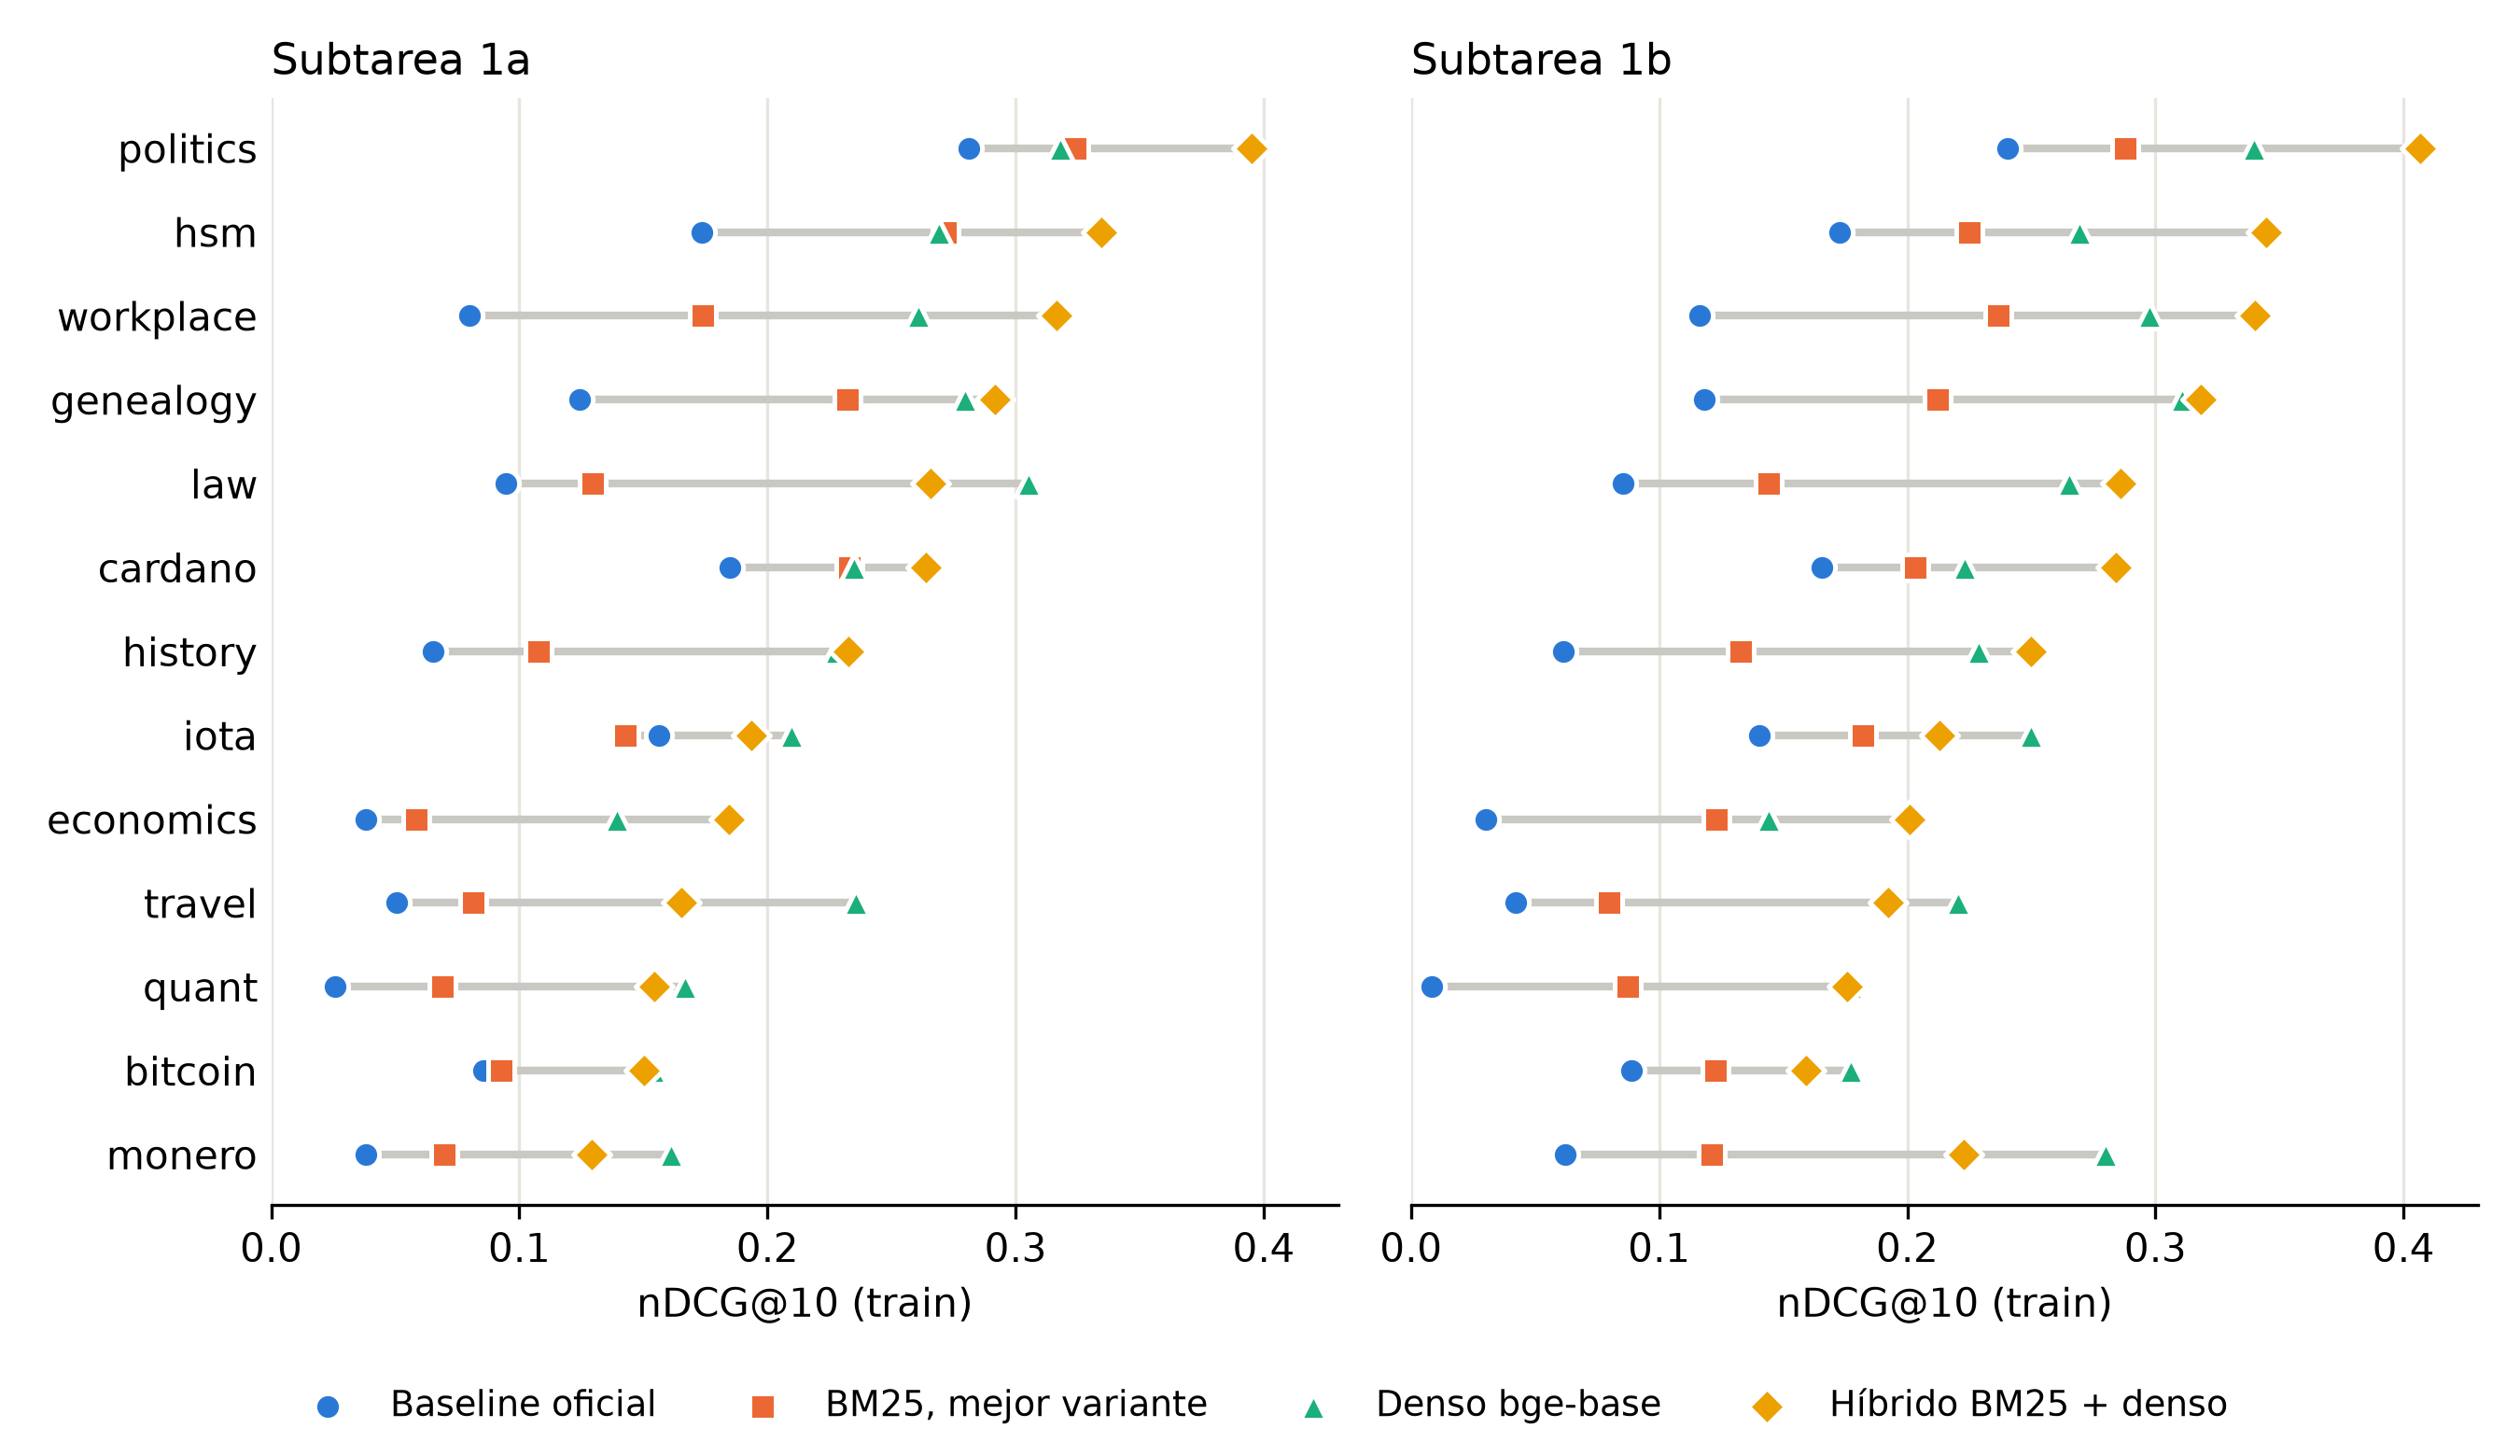
\includegraphics[width=\textwidth]{fig_dominios.png}
\caption{nDCG@10 por dominio de los cuatro sistemas de la tabla~\ref{tab:principal} (train). Los dominios están ordenados por el resultado del híbrido en 1a. La línea gris va del peor al mejor sistema en cada dominio. Las cifras están en la tabla~\ref{tab:dominios}.}
\label{fig:dominios}
\end{figure}

\subsection{Variantes de consulta con BM25}
\label{sec:res-variantes}

La tabla~\ref{tab:variantes} muestra que con BM25 \textbf{acortar la consulta es lo que más rinde}. El título solo supera a la consulta completa, y fusionar ambos con RRF es todavía mejor (+0.045, 12/13 dominios). En 1b, sustituir la consulta larga por el título y quitar al paso el verbo imperativo y las palabras meta mejora en los 13 dominios (+0.064). Es una mejora de 42~\% y 62~\% relativa sin ningún modelo, solo con expresiones regulares y la estructura de la consulta.

\begin{table}[t]
\centering
\caption{Variantes de consulta con BM25 (train). $\Delta$ y $p$ frente al baseline oficial; ``Dom.'' indica cuántos de los 13 dominios mejoran / empeoran.}
\label{tab:variantes}
\small
\begin{tabular}{llrrrrl}
\toprule
Sub. & Variante & nDCG@10 & R@1000 & $\Delta$ & $p$ & Dom. \\
\midrule
1a & \texttt{cruda} (oficial) & 0.1075 & 0.640 & --- & --- & --- \\
   & \texttt{limpia} & 0.1126 & 0.661 & +0.005 & 0.51 & 11/1 \\
   & \texttt{titulo+inicio} & 0.1347 & 0.686 & +0.027 & $<$0.001 & 12/1 \\
   & \texttt{titulo} & 0.1500 & 0.688 & +0.042 & $<$0.001 & 11/2 \\
   & \texttt{rrf(limpia,titulo)} & \textbf{0.1528} & \textbf{0.723} & +0.045 & $<$0.001 & 12/1 \\
\midrule
1b & \texttt{oficial} (consulta + paso) & 0.1024 & 0.701 & --- & --- & --- \\
   & \texttt{paso} & 0.1104 & 0.658 & +0.008 & 0.41 & 9/4 \\
   & \texttt{limpia+paso} & 0.1107 & 0.719 & +0.008 & 0.008 & 11/2 \\
   & \texttt{rrf(paso,limpia)} & 0.1432 & 0.768 & +0.041 & $<$0.001 & 13/0 \\
   & \texttt{titulo+paso} & 0.1611 & 0.779 & +0.059 & $<$0.001 & 13/0 \\
   & \texttt{titulo+paso\_limpio} & \textbf{0.1660} & \textbf{0.806} & +0.064 & $<$0.001 & 13/0 \\
\bottomrule
\end{tabular}
\end{table}

\subsection{Recuperador de embeddings}
\label{sec:res-denso}

El recuperador denso \textbf{duplica el baseline} y supera con holgura a la mejor variante de BM25: 0.2277 frente a 0.1528 en 1a y 0.2449 frente a 0.1660 en 1b, con mejora en los 13 dominios. El R@1000 sube a 0.863 y 0.917: el denso encuentra muchos relevantes que BM25 no ve. Al contrario que BM25, \textbf{el denso prefiere la consulta completa}: en 1a, la consulta limpia (0.2234) supera al título solo (0.2032), y en 1b el paso aislado se hunde (0.1155) frente a la consulta limpia más el paso (0.2449), como observa el paper de TEMPO. Lo que ayuda al denso es quitar el HTML, no acortar. Puntuar el documento por su mejor trozo apenas supera a usar solo el primer trozo (como mucho +0.007).

\subsection{Fusión híbrida}
\label{sec:res-hibrido}

La fusión \textbf{solo ayuda si BM25 pesa menos que el denso} (tabla~\ref{tab:hibrido}). Con pesos iguales no gana nada, porque BM25 es mucho más débil y mete ruido en las primeras posiciones. Con BM25 a peso 0.3--0.6 el resultado forma una meseta (0.234--0.239 en 1a y 0.258--0.261 en 1b), así que el riesgo de sobreajustar el peso es bajo, y fijamos $w = 0.5$. En 1b el híbrido cumple el criterio de aceptación frente al denso solo (+0.016, $p = 0.04$, 8/13 dominios); en 1a se queda cerca, sin significancia. En dev lo cumple en ambas subtareas (sección~\ref{sec:res-dev}). Fusionar las variantes oficiales de ambos recuperadores, en lugar de las mejores, empeora ($-0.027$ en 1b), así que la limpieza de la consulta sigue siendo necesaria. El híbrido también sube el recall (R@1000 de 0.917 a 0.939 en 1b).

\begin{table}[t]
\centering
\caption{Híbrido BM25 + denso con RRF ($k = 60$, train). $w$ es el peso de BM25 (el denso pesa 1). $\Delta$, $p$ y dominios frente al denso solo.}
\label{tab:hibrido}
\small
\begin{tabular}{llrrrrr}
\toprule
Sub. & Fusión & $w$ & nDCG@10 & $\Delta$ & $p$ & Dom. \\
\midrule
1a & denso solo & --- & 0.2277 & --- & --- & --- \\
   & BM25 + denso, mejores variantes & 1 & 0.2218 & $-$0.006 & 0.55 & 6/7 \\
   & ídem & 0.5 & \textbf{0.2367} & +0.009 & 0.21 & 7/6 \\
   & ídem & 0.4 & 0.2390 & +0.011 & 0.09 & 8/5 \\
\midrule
1b & denso solo & --- & 0.2449 & --- & --- & --- \\
   & BM25 + denso, mejores variantes & 1 & 0.2476 & +0.003 & 0.81 & 7/6 \\
   & ídem & 0.5 & \textbf{0.2610} & +0.016 & 0.04 & 8/5 \\
   & ídem & 0.4 & 0.2611 & +0.016 & 0.03 & 8/5 \\
   & BM25 + denso, variantes oficiales & 1 & 0.2180 & $-$0.027 & 0.007 & 4/9 \\
\bottomrule
\end{tabular}
\end{table}

Por dominio (tabla~\ref{tab:dominios}), el híbrido es el mejor sistema en 7 dominios en 1a y en 8 en 1b, con las mayores ganancias en \texttt{politics}, \texttt{hsm}, \texttt{economics} y \texttt{workplace}, mientras que en \texttt{travel}, \texttt{monero}, \texttt{quant} y \texttt{bitcoin} el denso solo es mejor en ambas subtareas.

\begin{table}[t]
\centering
\caption{nDCG@10 por dominio (train). $n$ es el número de consultas (1a) o pasos (1b). Base: baseline oficial; BM25: mejor variante; Denso: \texttt{bge-base}; Híbrido: BM25 (w 0.5) + denso.}
\label{tab:dominios}
\small
\begin{tabular}{lrrrrrrrrrr}
\toprule
 & \multicolumn{5}{c}{1a} & \multicolumn{5}{c}{1b} \\
Dominio & $n$ & Base & BM25 & Denso & Híbrido & $n$ & Base & BM25 & Denso & Híbrido \\
\midrule
bitcoin   & 70  & 0.086 & 0.093 & \textbf{0.154} & 0.150 & 132  & 0.089 & 0.123 & \textbf{0.177} & 0.159 \\
cardano   & 36  & 0.185 & 0.233 & 0.235 & \textbf{0.264} & 57   & 0.166 & 0.203 & 0.223 & \textbf{0.284} \\
economics & 58  & 0.038 & 0.058 & 0.139 & \textbf{0.185} & 130  & 0.030 & 0.123 & 0.144 & \textbf{0.201} \\
genealogy & 80  & 0.124 & 0.232 & 0.280 & \textbf{0.292} & 159  & 0.118 & 0.212 & 0.311 & \textbf{0.318} \\
history   & 561 & 0.065 & 0.108 & 0.228 & \textbf{0.233} & 1421 & 0.061 & 0.133 & 0.229 & \textbf{0.250} \\
hsm       & 105 & 0.174 & 0.272 & 0.269 & \textbf{0.335} & 254  & 0.173 & 0.225 & 0.269 & \textbf{0.345} \\
iota      & 7   & 0.156 & 0.143 & \textbf{0.210} & 0.193 & 16   & 0.140 & 0.182 & \textbf{0.250} & 0.213 \\
law       & 24  & 0.095 & 0.129 & \textbf{0.305} & 0.266 & 53   & 0.085 & 0.144 & 0.265 & \textbf{0.286} \\
monero    & 46  & 0.038 & 0.070 & \textbf{0.161} & 0.129 & 73   & 0.062 & 0.121 & \textbf{0.280} & 0.223 \\
politics  & 105 & 0.281 & 0.324 & 0.318 & \textbf{0.395} & 266  & 0.240 & 0.288 & 0.340 & \textbf{0.407} \\
quant     & 24  & 0.026 & 0.069 & \textbf{0.167} & 0.154 & 37   & 0.009 & 0.087 & \textbf{0.177} & 0.176 \\
travel    & 70  & 0.051 & 0.081 & \textbf{0.236} & 0.165 & 133  & 0.042 & 0.080 & \textbf{0.221} & 0.192 \\
workplace & 25  & 0.080 & 0.174 & 0.261 & \textbf{0.317} & 31   & 0.116 & 0.237 & 0.298 & \textbf{0.340} \\
\midrule
Macro     & 1211 & 0.108 & 0.153 & 0.228 & \textbf{0.237} & 2762 & 0.102 & 0.166 & 0.245 & \textbf{0.261} \\
\bottomrule
\end{tabular}
\end{table}

\subsection{Oráculos}
\label{sec:res-oraculos}

Con BM25, \textbf{añadir texto empeora}. Buscar con la respuesta aceptada real (O1, el HyDE ``perfecto'') da 0.0971 en 1a, por debajo del baseline: un texto largo diluye los términos, igual que la reformulación con LLM en el paper de TEMPO. Añadir las etiquetas temporales estructuradas (O2) apenas mueve el resultado (+0.005, no significativo). El resumen escrito por GPT-4o (O3) ayuda (+0.031), pero no supera al título solo (0.1500). Con el denso, añadir la respuesta real a la consulta limpia solo aporta +0.011 sobre \texttt{limpia} (0.2343 frente a 0.2234), y la respuesta sola empeora (0.1719). El margen de una reescritura con LLM es pequeño; lo que importa es \textbf{quitar ruido} a la consulta.

\subsection{Clasificación del tipo de razonamiento (O4, O5)}
\label{sec:res-razonamiento}

\paragraph{El clasificador es débil.} Con TF-IDF sobre unigramas y bigramas y regresión logística, la clase de razonamiento (7 clases) se predice con una exactitud de 0.47 y un macro-F1 de 0.33 (la clase mayoritaria da 0.36), y la intención con 0.43 y 0.38. Además, las etiquetas las generó un LLM y tienen ruido. Antes de mejorar el clasificador medimos si, con etiquetas perfectas, servía de algo (O4).

\paragraph{Ni con etiquetas perfectas el enrutamiento mejora.} Con las variantes de BM25 como candidatas, enrutar por clase queda en $-0.009$ (1a) y $+0.001$ (1b) frente a la mejor variante única: la misma variante gana en casi todas las clases. Al repetirlo con candidatos cualitativamente distintos (tabla~\ref{tab:o4}), el resultado es el mismo. Con validación cruzada, el enrutamiento por clase o intención queda entre $-0.005$ y $+0.000$ frente al híbrido. Elegir el peso de BM25 por grupo (candidatos suaves) tampoco ayuda, porque el barrido de pesos es una meseta para todos los grupos. Enrutar por dominio parece bueno en la muestra en la que se elige (+0.010 a +0.012), pero con validación cruzada queda en +0.005 en 1a ($p = 0.17$) y en $-0.003$ en 1b: es sobreajuste. El oráculo por consulta es alto (0.303 y 0.344), así que hay mucha variación entre consultas, pero ni la clase, ni la intención, ni el dominio la explican.

\begin{table}[t]
\centering
\caption{O4 repetido: enrutamiento con validación cruzada de 5 particiones (train). Candidatos duros: BM25, denso o híbrido; suaves: el híbrido con el peso de BM25 en 0.2--0.7 o 1. $\Delta$ frente a la mejor estrategia única de cada conjunto (híbrido con $w = 0.5$ en el duro, $w = 0.4$ en el suave).}
\label{tab:o4}
\footnotesize
\setlength{\tabcolsep}{4pt}
\begin{tabular}{llrrrr}
\toprule
Agrupación & Candidatos & 1a & $\Delta$ ($p$) & 1b & $\Delta$ ($p$) \\
\midrule
Mejor estrategia única & duro / suave & 0.2367 / 0.2390 & --- & 0.2610 / 0.2611 & --- \\
Clase & duro & 0.2372 & +0.000 (0.78) & 0.2604 & $-$0.001 (0.57) \\
Clase & suave & 0.2370 & $-$0.002 (0.18) & 0.2615 & +0.000 (0.88) \\
Intención & duro & 0.2344 & $-$0.002 (0.49) & 0.2561 & $-$0.005 (0.13) \\
Intención & suave & 0.2342 & $-$0.005 (0.04) & 0.2614 & +0.000 (0.91) \\
Dominio & duro & 0.2417 & +0.005 (0.17) & 0.2577 & $-$0.003 (0.43) \\
Dominio & suave & 0.2397 & +0.001 (0.85) & 0.2600 & $-$0.001 (0.74) \\
\midrule
Oráculo por consulta & duro / suave & 0.3030 / 0.2734 & & 0.3436 / 0.3039 & \\
\bottomrule
\end{tabular}
\end{table}

\paragraph{No hay un vocabulario de documento por clase (O5).} De 37 pistas escritas a mano (por ejemplo, ``circa'' o ``museum'' para la clase de materiales y procedencia), solo ``century'' resulta significativa en una clase ($z = 3.5$), y ``museum'' sale incluso negativa ($z = -2.4$). Los términos característicos de cada clase son temáticos (``troops'', ``soviet'', ``utxo''): reflejan los dominios y los temas, no el tipo de razonamiento. La única señal fuerte es común a todas las clases: los \emph{hard negatives} son páginas bibliográficas o editoriales (``copyright'', ``press'', ``university'', ``library''), y los relevantes son texto narrativo o enciclopédico.

\subsection{K4: década y siglo}
\label{sec:res-k4}

El 45~\% de las consultas de 1a y de los pasos de 1b tiene alguna fecha (93--94~\% en \texttt{genealogy}, 0~\% en \texttt{iota}). La tabla~\ref{tab:k4} muestra que K4 no cumple el criterio en ningún caso. Añadir las formas al texto (a) empeora BM25 de forma significativa ($-0.007$ en 1a y $-0.006$ en 1b, $p < 0.001$), sobre todo en \texttt{genealogy}, donde las consultas tienen muchas fechas. Hay dos causas: el \emph{stemmer} convierte ``1830s'' en ``1830'', un año que no estaba en la consulta, y ``19th century'' acerca cualquier documento del siglo. En el híbrido, (a) y (b) se mueven entre $-0.003$ y $+0.004$. La pequeña subida de (b) en 1b viene de añadir un texto más a la fusión, no de las formas: el control, sin las formas, sube lo mismo.

\begin{table}[t]
\centering
\caption{K4 sobre el híbrido (train). $\Delta$ y $p$ frente al híbrido base. (a) formas añadidas a la consulta; (b) texto extra con las formas, fusionado con RRF; control: el mismo texto extra sin las formas.}
\label{tab:k4}
\footnotesize
\setlength{\tabcolsep}{4pt}
\begin{tabular}{lrrrrr}
\toprule
Sub. & Base & (a) & (b) & Control & (b) $-$ control \\
\midrule
1a & 0.2367 & 0.2340 ($-$0.003, $p$ 0.28) & 0.2348 ($-$0.002, $p$ 0.35) & 0.2346 ($-$0.002, $p$ 0.28) & +0.000 \\
1b & 0.2610 & 0.2608 ($-$0.000, $p$ 0.85) & 0.2652 (+0.004, $p$ 0.04) & 0.2657 (+0.005, $p$ 0.02) & $-$0.000 \\
\bottomrule
\end{tabular}
\end{table}

\subsection{TT0: perfil temporal implícito}
\label{sec:res-tt0}

\paragraph{El léxico capta periodos reales.} Los léxicos tienen entre 58 mil y 114 mil n-gramas, aprendidos de 1.4--3.2~M oraciones por dominio, de las que entre el 18~\% y el 22~\% tienen fecha. Los n-gramas más específicos apuntan al periodo correcto aunque el año no esté en la oración: ``henry viii'' $\rightarrow$ década de 1530, ``glorious revolution'' $\rightarrow$ década de 1680, ``qin dynasty'' $\rightarrow$ siglo III a.\,C., ``etruscans'' $\rightarrow$ siglo VII a.\,C. Pero también hay mucho ruido: páginas repetidas, plantillas de citas y números que no son años. Los n-gramas que más aparecen en oraciones fechadas son metadatos (``accessed june'', ``archived november''), igual que en O5.

\paragraph{La señal es débil y solo existe en los dominios históricos.} La tabla~\ref{tab:tt0} muestra que la similitud temporal separa relevantes de no relevantes con un AUC de 0.60--0.65 en \texttt{history} y \texttt{hsm}, y casi al azar en \texttt{politics}. En \texttt{history} 1b, el perfil implícito llega a 0.635 en 565 pasos sin ninguna fecha explícita: ni el extractor ni K4 pueden decir nada de esos pasos. Pero dentro del mismo grupo de candidatos, el score del propio híbrido separa con un AUC de 0.77--0.89.

\paragraph{La fusión gana algo, pero no es estable.} Fusionar el orden temporal con el del híbrido sube +0.007 a +0.011 en \texttt{history} y \texttt{hsm}, y baja en \texttt{politics}. Sin embargo, la mejor combinación se elige entre 9 en el propio dominio, cambia entre 1a y 1b y, aplicada en la otra subtarea, queda entre $-0.003$ y $+0.005$. Aunque se aplicara solo en esos dos dominios, el efecto en la macro sería de unas $+0.001$--$0.002$. No la adoptamos.

\begin{table}[t]
\centering
\caption{TT0 dentro de los 100 primeros del híbrido (train). AUC medio por consulta (0.5 = azar) con los perfiles explícito (E), implícito (I) y mixto (EI). ``Mejor fusión'': mejor nDCG@10 de 9 combinaciones (perfil $\times$ peso), elegida en el propio dominio, por lo que es optimista.}
\label{tab:tt0}
\small
\begin{tabular}{llrrrrrrl}
\toprule
Dominio & Sub. & $n$ & AUC E & AUC I & AUC EI & AUC híbrido & Base & Mejor fusión \\
\midrule
politics & 1a & 105  & 0.491 & 0.530 & 0.483 & 0.83--0.85 & 0.3952 & 0.3945 ($-$0.001) \\
politics & 1b & 266  & 0.524 & 0.571 & 0.525 & 0.89 & 0.4067 & 0.4019 ($-$0.005) \\
history  & 1a & 561  & 0.631 & 0.620 & 0.622 & 0.77--0.78 & 0.2323 & 0.2420 (+0.010) \\
history  & 1b & 1421 & 0.645 & 0.636 & 0.640 & 0.82 & 0.2499 & 0.2608 (+0.011) \\
hsm      & 1a & 105  & 0.636 & 0.601 & 0.593 & 0.82--0.85 & 0.3347 & 0.3435 (+0.009) \\
hsm      & 1b & 254  & 0.635 & 0.603 & 0.596 & 0.82 & 0.3445 & 0.3511 (+0.007) \\
\bottomrule
\end{tabular}
\end{table}

\subsection{Comprobación en dev}
\label{sec:res-dev}

Al final del proyecto corrimos una sola vez en dev los cuatro sistemas de la tabla~\ref{tab:principal}, con la configuración fijada en train: las mismas variantes de consulta, RRF con $k = 60$ y BM25 con peso 0.5. No se ajustó nada después. Dev tiene 519 consultas (1a) y 1,214 pasos (1b) de los mismos 13 dominios, distintos de los de train. K4, TT0 y el enrutamiento de O4 no se evaluaron en dev, porque no se adoptaron.

La tabla~\ref{tab:dev} muestra que \textbf{la progresión de train se repite en dev}. El híbrido llega a 0.2519 en 1a y 0.2971 en 1b, 2.2 y 2.5 veces el baseline, con cifras incluso algo mejores que en train. Cada paso mejora al anterior de forma significativa. En particular, el híbrido supera al denso solo en +0.029 en 1a ($p < 0.001$, 9/13 dominios) y en +0.036 en 1b ($p < 0.001$, 11/13), así que en dev cumple el criterio de aceptación en las dos subtareas, mientras que en train solo lo cumplía en 1b. Frente al baseline, el híbrido mejora en 12 de 13 dominios en 1a y en los 13 en 1b. La única excepción es \texttt{quant} en 1a, con 10 consultas en dev, donde todos los sistemas quedan por debajo de 0.04.

\begin{table}[t]
\centering
\caption{Comprobación única en dev de los sistemas de la tabla~\ref{tab:principal}, con la configuración fijada en train. $\Delta$ frente a la fila anterior, con el $p$ del test pareado y los dominios que mejoran / empeoran. La última columna repite el nDCG@10 de train para comparar.}
\label{tab:dev}
\footnotesize
\setlength{\tabcolsep}{4pt}
\begin{tabular}{llrrrrr}
\toprule
Sub. & Sistema & nDCG@10 & $\Delta$ ($p$; dom.) & R@100 & R@1000 & Train \\
\midrule
1a & Baseline oficial & 0.1147 & --- & 0.404 & 0.660 & 0.1075 \\
   & BM25, \texttt{rrf(limpia,titulo)} & 0.1716 & +0.057 ($<$0.001; 11/2) & 0.518 & 0.772 & 0.1528 \\
   & Denso \texttt{bge-base} & 0.2226 & +0.051 (0.002; 8/5) & 0.660 & 0.893 & 0.2277 \\
   & \textbf{Híbrido BM25 (w 0.5) + denso} & \textbf{0.2519} & +0.029 ($<$0.001; 9/4) & \textbf{0.692} & \textbf{0.900} & 0.2367 \\
\midrule
1b & Baseline oficial & 0.1177 & --- & 0.443 & 0.716 & 0.1024 \\
   & BM25, \texttt{titulo+paso\_limpio} & 0.1838 & +0.066 ($<$0.001; 11/2) & 0.556 & 0.807 & 0.1660 \\
   & Denso \texttt{bge-base} & 0.2610 & +0.077 ($<$0.001; 12/1) & 0.750 & 0.922 & 0.2449 \\
   & \textbf{Híbrido BM25 (w 0.5) + denso} & \textbf{0.2971} & +0.036 ($<$0.001; 11/2) & \textbf{0.779} & \textbf{0.939} & 0.2610 \\
\bottomrule
\end{tabular}
\end{table}

\begin{table}[t]
\centering
\caption{nDCG@10 por dominio en dev. $n$ es el número de consultas (1a) o pasos (1b). Mismas columnas que la tabla~\ref{tab:dominios}. Los dominios con menos de 15 consultas (\texttt{iota}, \texttt{law}, \texttt{quant}, \texttt{workplace} en 1a) son muy ruidosos.}
\label{tab:dominios-dev}
\small
\begin{tabular}{lrrrrrrrrrr}
\toprule
 & \multicolumn{5}{c}{1a} & \multicolumn{5}{c}{1b} \\
Dominio & $n$ & Base & BM25 & Denso & Híbrido & $n$ & Base & BM25 & Denso & Híbrido \\
\midrule
bitcoin   & 30  & 0.037 & 0.094 & 0.187 & \textbf{0.239} & 56  & 0.030 & 0.118 & 0.243 & \textbf{0.262} \\
cardano   & 15  & 0.103 & 0.102 & 0.132 & \textbf{0.189} & 33  & 0.063 & 0.119 & 0.168 & \textbf{0.212} \\
economics & 25  & 0.047 & 0.041 & 0.151 & \textbf{0.183} & 51  & 0.046 & 0.119 & 0.179 & \textbf{0.219} \\
genealogy & 35  & 0.195 & 0.275 & 0.250 & \textbf{0.304} & 68  & 0.218 & 0.211 & 0.301 & \textbf{0.369} \\
history   & 240 & 0.087 & 0.119 & \textbf{0.260} & 0.249 & 636 & 0.102 & 0.179 & 0.282 & \textbf{0.291} \\
hsm       & 45  & 0.249 & 0.364 & 0.338 & \textbf{0.415} & 105 & 0.214 & 0.256 & 0.240 & \textbf{0.350} \\
iota      & 3   & 0.331 & \textbf{0.450} & 0.327 & 0.347 & 8   & 0.420 & 0.362 & 0.460 & \textbf{0.498} \\
law       & 11  & 0.057 & 0.117 & \textbf{0.208} & 0.206 & 23  & 0.055 & 0.187 & 0.288 & \textbf{0.303} \\
monero    & 19  & 0.032 & 0.070 & 0.144 & \textbf{0.160} & 28  & 0.011 & 0.029 & 0.119 & \textbf{0.186} \\
politics  & 45  & 0.263 & 0.391 & 0.358 & \textbf{0.483} & 119 & 0.237 & 0.275 & 0.297 & \textbf{0.404} \\
quant     & 10  & 0.024 & \textbf{0.039} & 0.000 & 0.019 & 15  & 0.040 & 0.086 & 0.108 & \textbf{0.112} \\
travel    & 30  & 0.044 & 0.071 & \textbf{0.211} & 0.162 & 52  & 0.065 & 0.185 & \textbf{0.258} & 0.212 \\
workplace & 11  & 0.023 & 0.100 & \textbf{0.328} & 0.320 & 20  & 0.030 & 0.263 & \textbf{0.451} & 0.444 \\
\midrule
Macro     & 519 & 0.115 & 0.172 & 0.223 & \textbf{0.252} & 1214 & 0.118 & 0.184 & 0.261 & \textbf{0.297} \\
\bottomrule
\end{tabular}
\end{table}

% -----------------------------------------------------------------------------
\section{Discusión}
\label{sec:discusion}

\paragraph{Cómo mejoramos las métricas.} La mejora total sobre el baseline es de +0.129 en 1a (de 0.1075 a 0.2367, +120~\%) y de +0.159 en 1b (de 0.1024 a 0.2610, +155~\%), y el R@1000 sube de 0.640 a 0.870 y de 0.701 a 0.939. Se reparte en tres pasos:
\begin{enumerate}
  \item \textbf{Limpiar la consulta} con expresiones regulares (+0.045 / +0.064): quitar el HTML, quedarse con el título y quitar al paso las palabras que no aparecen en los documentos. Ataca la dilución de los términos clave en consultas largas.
  \item \textbf{Embeddings} (+0.075 / +0.079 sobre la mejor variante de BM25): resuelven buena parte del desajuste de vocabulario que mostró el análisis exploratorio, porque encuentran documentos que hablan del tema con otras palabras.
  \item \textbf{Fusión con BM25 a medio peso} (+0.009 / +0.016 sobre el denso): BM25 aporta la coincidencia exacta de nombres propios, años y términos técnicos, que el denso a veces pierde, siempre que no pese tanto como para meter ruido arriba.
\end{enumerate}
Cada paso exige elegir bien la variante de consulta de cada recuperador: BM25 quiere textos cortos y el denso textos completos y limpios. En dev la progresión se repite con la configuración fijada en train: de 0.1147 a 0.2519 en 1a (+120~\%) y de 0.1177 a 0.2971 en 1b (+152~\%), con aportes de +0.057 / +0.066 por la limpieza, +0.051 / +0.077 por los embeddings y +0.029 / +0.036 por la fusión. Que la fusión aporte incluso más en dev que en train sugiere que el peso de BM25 elegido en train no estaba sobreajustado.

\paragraph{Por qué el tiempo explícito no ayuda.} Probamos cuatro formas de usar el tiempo o el tipo de razonamiento, y ninguna mejora el híbrido de forma estable. La explicación común es que \textbf{los candidatos del híbrido ya comparten tema y época con la consulta}. Añadir la década o el siglo (K4) no distingue entre documentos que hablan del mismo periodo, y el perfil implícito (TT0) fecha ``la época'' con un error de décadas, como ya observaban \citet{jatowt2013focus}, justo lo que el híbrido ya comparte. El tipo de razonamiento tampoco decide qué estrategia conviene (O4): la fusión ya absorbe las diferencias entre recuperadores. Lo que distingue a un documento relevante dentro del grupo de candidatos es otra cosa: que responda a la pregunta y que sea contenido narrativo, no una página bibliográfica (O5). Esto es coherente con TEMPO, donde quitar las expresiones temporales de la consulta apenas cambia el resultado de los recuperadores.

\paragraph{Limitaciones.} Las decisiones se tomaron en train y dev se usó una sola vez. Dev confirma los resultados, pero comparte dominios y corpus con train y no sustituye al test oficial, cuyos juicios de relevancia no son públicos. Los dominios pequeños son muy ruidosos: \texttt{iota} tiene 7 consultas en train y 3 en dev, y pesa 1/13 de la macro. Los juicios de relevancia son incompletos: en la revisión manual, el primer documento recuperado a menudo era relevante sin estar marcado. Nuestras cifras no son directamente comparables con las del paper de TEMPO, que evalúa sobre train y dev juntos y con el corpus anterior a la deduplicación. Por último, la codificación densa en GPU no es del todo determinista (diferencias de $\pm$0.0005).

% -----------------------------------------------------------------------------
\section{Conclusiones y trabajo futuro}

Con técnicas de la materia y sin ningún modelo de lenguaje generativo, el sistema híbrido BM25 + embeddings con BM25 a medio peso alcanza un macro nDCG@10 de 0.2367 en 1a y 0.2610 en 1b en train, 2.2 y 2.5 veces el baseline oficial. La comprobación única en dev lo confirma (0.2519 y 0.2971), y allí el híbrido supera al denso solo de forma significativa en ambas subtareas. Las mayores ganancias vienen de limpiar la consulta y de añadir un recuperador semántico, no de modelar el tiempo. Clasificar el tipo de razonamiento, buscar vocabulario por clase, añadir formas temporales gruesas y estimar el periodo implícito con n-gramas y una cadena de Markov no mejoran de forma estable el sistema, por razones que el análisis permite explicar.

Como trabajo futuro quedan: penalizar las páginas bibliográficas (la señal más fuerte de O5); probar en todos los pasos de 1b el texto extra ``título. paso limpio'' en el brazo denso, que dio +0.005 ($p = 0.02$) como efecto secundario de K4; y, si se retoma TT0, elegir la fusión con validación cruzada en los dominios históricos.

% -----------------------------------------------------------------------------
\bibliographystyle{plainnat}
\bibliography{referencias}

\end{document}
